% chapter3.tex
% Capitulo 3. Estudio de la plataforma USRP y GNURadio
%==========================================================================
\chapter{Estudio de la plataforma USRP y GNURadio}
\label{ch:estudio}

En este cap\'itulo se aplican los conceptos de la modulaci\'on QPSK para
analizar el rendimiento de la plataforma USRP. El experimento consta de elaborar
un programa que realice la modulaci\'on utilizando el lenguaje Python y
\gnuradio\ bajo el ambiente Linux. Este programa va interactuar con el USRP
por medio del puerto USB, intercambiando la informaci\'on que se transmite y
recibe. El an\'alisis ser\'a visualizado en la PC utilizando las herramientas
que \gnuradio\ proporciona.

La transmisi\'on se realizar\'a utilizando las tarjetas LFTX y LFRX. Estas
tarjetas proporcionan acceso directo a las salidas del DAC y entradas del ADC
respectivamente sin ning\'un tipo de amplificaci\'on y filtrado. Dependiendo la
aplicaci\'on ser\'a necesario acoplar una etapa de RF para acondicionar la
se\~nal y poder ser transmitida correctamente.

% 3.1. Estructura del sistema USRP
%==========================================================================
\section{Estructura del sistema USRP}

El sistema USRP es un dispositivo que permite dise\~nar radios reconfigurables
por software. El dispositivo es solamente una parte de la estructura completa de
un SDR. Su funci\'on principal es actuar como la secci\'on de frecuencia intermedia de un sistema de
comunicaciones.

La figura \ref{fig:sisusrp} muestra los componentes que forman un sistema de
comunicaciones implementado con el USRP. Todo el procesamiento en banda base, es decir,
modulaciones, codificaciones, etc., es llevado a cabo en una PC x86. Esta PC
contiene el programa Python que realiza todo el procesamiento digital con la
se\~nal o se\~nales que se desean trabajar. Esto se lleva a cabo utilizando las
herramientas proporcionadas por \gnuradio.

\begin{figure}[t]
\centering
	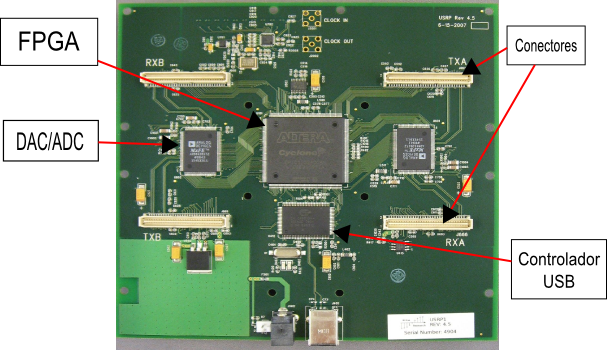
\includegraphics[width=5.5in]{figs/usrp}
	\vspace{0.3in}
	\caption{Placa principal del USRP.}
	\label{fig:sisusrp}
\end{figure}

Los componentes principales del USRP son el FPGA Altera Cyclone EP1C12, los codec AD9862 de alta
velocidad , las interfaces de las tarjetas auxiliares y el controlador Cypress FX2 para la
comunicaci\'on por el puerto USB. La tarjeta cuenta con 4 conectores donde se pueden conectar 2
tarjetas TX y 2 RX o 2 tarjetas RFX (transmisor y receptor en una sola tarjeta auxiliar). Cada
tarjeta puede acceder a dos de los 4 ADC/DACs. Si la tarjeta utiliza muestreo real (sin usar IQ)
entonces esto permitir\'a tener 2 secciones de RF independientes, para un total de 4. Si se utiliza
muestreo complejo IQ entonces cada tarjeta tendra una sola etapa de RF, para un total de 2 en todo
el sistema. Cada tarjeta auxiliar tiene dos conectores SMA para transmitir o recibir se\~nales y una
EEPROM con bus de datos I\textsuperscript{2}C que identifica la tarjeta al sistema. Esto permite que el software en la
PC pueda configurar el sistema bas\'andose en la tarjeta que este instalada. Las tarjetas que
actualmente soporta el USRP se muestran en la tabla \ref{tbl:cards}.

\begin{table}[htp]
\begin{center}
	\begin{tabular}{|c|p{8cm}|p{3cm}|}
		\hline
		\textbf{Tarjeta} & \textbf{Descripci\'on} & \textbf{Frecuencia de operaci\'on}\\
		\hline
		BasicTX y RX & Transmisor y Receptor para ser utilizados con equipo externo de RF. Sus salidas
		estan acopladas por un transformador directamente a los ADC/DACs con una impedancia de 50$\Omega$.
		& 1Mhz-250Mhz\\
		\hline
		LFTX y LFRX & Similar al BasicTX y RX pero las salidas estan acopladas por amplificadores
		diferenciales en lugar de transformadores. Esto las permite trabajar con frecuencias hasta DC.
		Tambi\'en cuentan con un filtro pasabajas con frecuencia de corte de 30Mhz. & DC-30Mhz\\
		\hline
		TVRX & Sistema receptor de VHF y UHF basando en un sintonizador de TV con un ancho de banda de
		canal de 6Mhz. & 50Mhz-860Mhz\\
		\hline
		DBSRX & Sistema receptor con filtro de canal controlado por software de 1Mhz a 60Mhz. &
		800Mhz-2.4Ghz\\
		\hline
		RFX400 & TX y RX en una sola tarjeta con un ancho de banda de canal de 30Mhz. & 400Mhz-500Mhz\\
		\hline
		RFX900 & TX y RX con 200mW(23dBm) de potencia.  & 750Mhz-1050Mhz\\
		\hline
		RFX1200 & TX y RX con 200mW de potencia que cubre las bandas satelitales. & 1150Mhz-1450Mhz\\
		\hline
		RFX1800 & TX y RX con 100mW(20dBm) de potencia & 1.5Ghz-2.1Ghz\\
		\hline
		RFX2400 & TX y RX con 50mW(17dBm) de potencia con un filtro pasabandas alrededor de la banda
		ISM(2400-2433Mhz). El filtro se puede deshabilitar para utilizar todo el rango de frecuencias. &
		2.3Ghz-2.9Ghz\\
		\hline
		XCVR2450 & TX y RX que cubre toda la banda ISM asi como tambi\'en algunas bandas japonesas. &
		2.4-2.5Ghz y 4.9-5.9Ghz\\
		\hline
		WBX & TX y RX que cubre varias bandas incluyendo televisi\'on, comunicaciones m\'obiles, sensores
		inal\'ambricos, etc. & 50Mhz-2.2Ghz\\
		\hline
	\end{tabular}
	\vspace{0.5in}
	\caption{Tarjetas auxiliares que soporta el USRP.}
	\label{tbl:cards}
\end{center}
\end{table}

El controlador FX2 integra un CPU 8051 con un controlador de USB de alta velocidad que implementa 3
\emph{endpoints} l\'ogicos para la comunicaci\'on con el FPGA y la PC como se describen en la tabla
\ref{tbl:endpoints}. Cada \emph{endpoint} establece una v\'ia de comunicaci\'on entre el dispostivo
USB y el \emph{host}. El endpoint 0 es el de control y es necesaria su implementaci\'on para que el
dispositivo pueda ser compatible y a su vez, ser certificado por el est\'andar de USB \cite{usb}.
Los endpoints 2 y 6 son de tipo Bulk, que de acuerdo a la especificaci\'on del USB, son los que
permiten el mayor rendimiento de transferencia (512 bytes por paquete). Estos son utilizados para
enviar los datos de la se\~nal al FPGA. El FX2 utiliza una interfaz de prop\'osito gen\'erico (GPIF)
para proporcionar un bus de datos al mundo exterior, esto con el prop\'osito de facilitar la
interfaz a otros dispositivos. En este caso el GPIF se conecta directamente al FPGA con una tasa de
transferencia de 96 MB/sec.

\begin{table}[htp]
\begin{center}
	\begin{tabular}{|c|c|}
		\hline
		\textbf{Endpoints} & \textbf{Descripci\'on} \\
		\hline
		0 & Control/Status \\
		\hline
		2 & PC $\rightarrow$ FPGA \\
		\hline
		6 & FPGA $\rightarrow$ PC \\
		\hline
	\end{tabular}
	\vspace{0.5in}
	\caption{\emph{Endpoints} implementados por el controlador FX2}
	\label{tbl:endpoints}
\end{center}
\end{table}

El FPGA es el encargado de realizar operaciones de alta velocidad y de reducir
la tasa de datos en una m\'as adecuada para que la se\~nal pueda ser transferida
por el puerto USB. Para la etapa de RX, la configuraci\'on b\'asica contiene dos
convertidores digitales hacia abajo (DDC) implementados con filtros CIC (Peine
Integradores en Cascada) de 4 etapas y filtros de media banda (\emph{Half-band}
o HB) de orden 31. El prop\'osito del DDC es transformar la se\~nal pasa bandas a banda base. Esto
se logra centrando su frencuencia en 0Hz, as\'i eliminando la portadora. La estructura del
DDC se muestra en la figura \ref{fig:ddcblock}.

\begin{figure}[htp]
\centering
	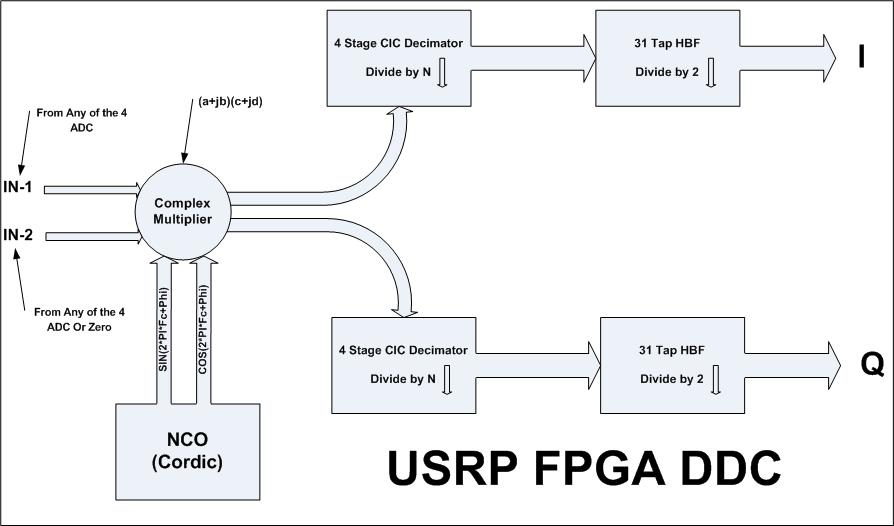
\includegraphics[width=5.5in]{figs/ddc}
	\vspace{0.3in}
	\caption{Estructura del DDC implementado en el USRP}
	\label{fig:ddcblock}
\end{figure}

EL USRP, en su configuraci\'on b\'asica, usa dos DDCs, cada uno con 2
entradas. La se\~nal compleja que entregan los ADCs es multiplicada por otra se\~nal con una
frecuencia intermedia constante generada por un oscilador controlado num\'ericamente (NCO).  La
se\~nal resultante se encuentra ahora centrada en 0Hz. Despu\'es es introducida al filtro CIC para
realizar una decimaci\'on por $N$, donde $N$ es especificado por el usuario desde el programa
del usuario. La funci\'on de transferencia del filtro CIC en el dominio $Z$ es la siguiente
\cite{cic}:

\begin{equation}\label{eq:cic}
H(z)=H_I^N(z)H_C^N(z)=\frac{(1-z^{-RM})^N}{(1-z^{-1})^N}=\left(\sum_{k=0}^{RM-1}z^{-1}\right)^N
\end{equation}

\begin{equation*}
\begin{aligned}
\text{Donde: }H_I^N&=\text{es la funci\'on de transferencia de la etapa
integradora}\\
H_C^N&=\text{es la funci\'on de transferencia de la etapa filtro comb}\\
R&=\text{es la tasa de decimaci\'on o interpolaci\'on}\\
M&=\text{n\'umero de muestras por etapa}\\
N&=\text{n\'umero de etapas por filtro}
\end{aligned}
\end{equation*}

Como aclaraci\'on, la variable $Z$ en la ecuaci\'on \ref{eq:cic} no es la misma que la ecuaci\'on \ref{eq:demgauss} ya que en la
ecuaci\'on anterior se refiere a la transformada Z y en la segunda ecucaci\'on se refiere a un proceso estoc\'astico.
El USRP implementa este filtro con los siguientes par\'ametros: $R$ = variable (4 m\'inimo), $M$ = 1 y $N$ = 4. La respuesta a la
frecuencia de esta configuraci\'on se muestra en la figura \ref{fig:cicresp}.

\begin{figure}[tp]
\centering
	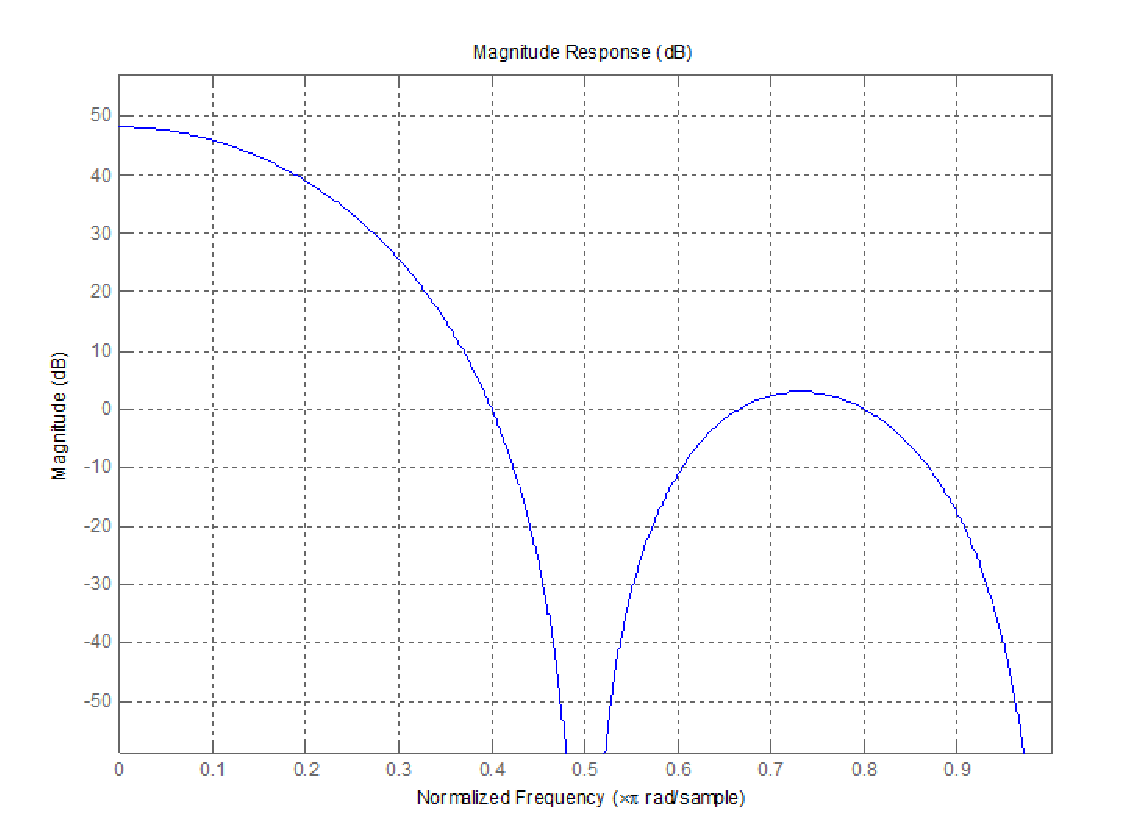
\includegraphics[width=5.9in]{figs/cicresponse}
	\caption{Respuesta a la frecuencia del filtro CIC de 4 etapas y R =	4}
	\label{fig:cicresp}
\end{figure}

La \'ultima etapa del DDC es el filtro HB el cual realiza una decimaci\'on de 2
y ayuda a rechazar cualquier banda no deseada por las operaciones previas. La
funci\'on de transferencia del filtro HB \cite{nguyen} es la
siguiente:

\begin{equation}
H(z)=\sum_{n=0}^{N-1}h(n)z^{-n}
\end{equation}

Estos filtros tienen las siguientes restricciones:

\begin{itemize}
  \item N-1 debe ser par
  \item $h(n)=h(N-1-n)$
\end{itemize}

La respuesta a la frecuencia es

\begin{equation}
H(e^{j\omega})=e^{-j\omega N-1/2}H_0(e^{-j\omega})
\end{equation}

donde $H_0(e^{-j\omega})$ representa la respuesta a la amplitud con valor real.

\begin{figure}[pt]
\centering
	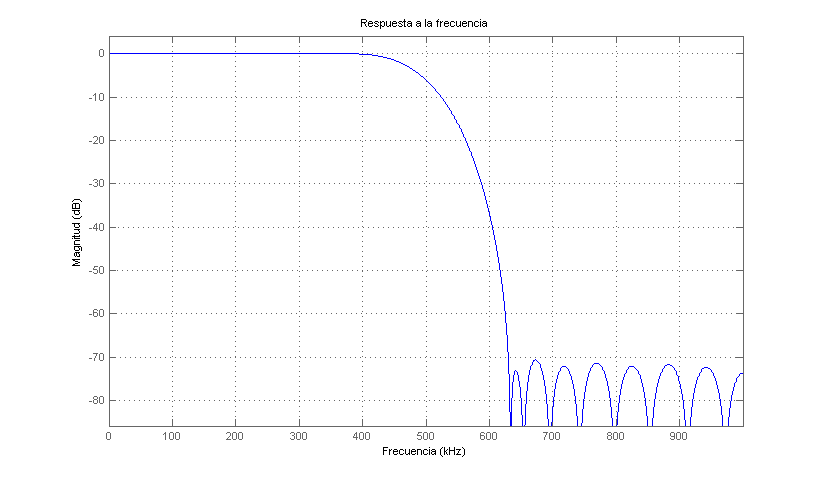
\includegraphics[width=5.9in]{figs/hbresponse}
	\caption{Respuesta a la frecuencia del filtro de media banda}
	\label{fig:hbresp}
\end{figure}

Las caracter\'isticas del filtro HB de acuerdo al USRP son las siguientes:

\begin{itemize}
  \item Orden 31
  \item Decimador 2
  \item Pasa bajas
\end{itemize}

En la figura \ref{fig:hbresp} se muestra la respuesta a la frecuencia del filtro HB.
Existe simetr\'ia con respecto a la banda $\pi /2$. Esta es una de las
caracter\'isticas de estos filtros. Debido a esa simetr\'ia la respuesta al
impulso es

\begin{equation}
h(n)=\left\{
\begin{array}{l l}
0, & \quad n=\frac{N-1}{2}=\text{par y diferente a 0}\\
\frac{1}{2}, & \quad n=\frac{N-1}{2}
\end{array}\right.
\end{equation}

Debido a esta simetr\'ia estos filtros son muy eficientes y f\'aciles de
implementar ya que aproximadamente el 50\% de sus coeficientes son 0.

La combinaci\'on del filtro CIC y HB dan un factor de decimaci\'on m\'inimo de
8. El ADC tiene una taza de muestreo de 64Ms/S, por lo tanto, el ancho de banda
total ser\'a de 32Mhz. Los datos enviados son de 16 bits para I y Q, \'osea, 4
bytes por muestra compleja. Esto resulta en un ancho de banda efectivo de 8Mhz
(32Mhz/4bytes). El rango de decimaci\'on que soporta el USRP es [8, 256]. El ancho de banda de la se\~nal no es afectado por la
operaci\'on de decimaci\'on, unicamente su frecuencia. Conforme el valor de decimaci\'on es mayor la taza de transferencia ser\'a
menor. El usuario puede ajustar este valor seg\'un las necesidades de su aplicaci\'on.

Para la etapa de TX el proceso es el inverso. El FPGA contiene filtros CIC interpoladores que se
encargan de interpolar la se\~nal, elevarla a la frecuencia intermedia y despu\'es
enviarla a los DACs. El proceso de conversi\'on digital hacia arriba (DUC)
est\'a contenido en el chip AD9862 y no en el FPGA como lo es en el proceso de
RX. Este chip contiene ambos ADCs y DACs pero \'unicamente en la etapa del TX
realiza alg\'un otro procesamiento sobre la se\~nal. La frecuencia de muestreo
de los DACs es de 128MS/s de 14 bits cada uno, d\'andonos una frecuencia Nyquist
de 64MS/s. La salida proporciona 1V pico a una carga diferencial de 50$\Omega$.
Existe un amplificador de ganancia programable (PGA) que puede proporcionar
hasta 20dB de ganancia y es programable por software. Las se\~nales del DAC son
en base a corriente y varean entre 0 y 20mA.

% \begin{figure}[hpt]
% \centering
% 	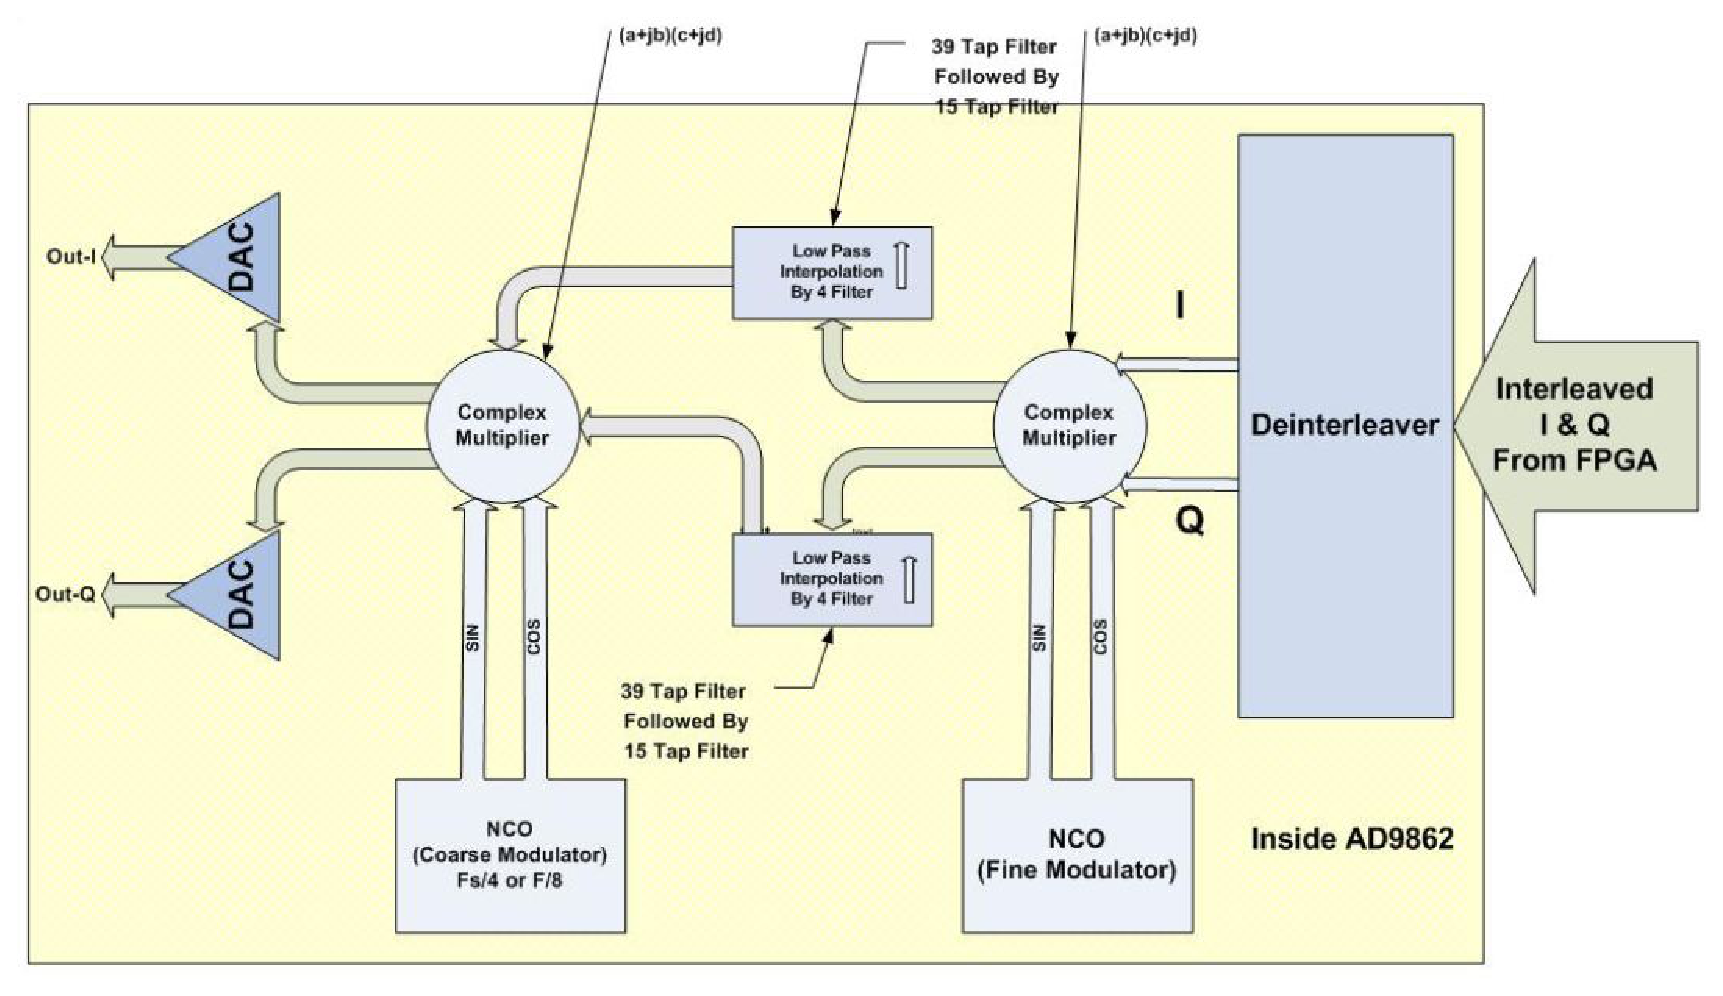
\includegraphics[width=5.5in]{figs/duc}
% 	\vspace{0.2in}
% 	\caption{Estructura del DUC implementado en el AD9862}
% 	\label{fig:ducblock}
% \end{figure}

% 3.2. GNURadio
%==========================================================================
\section{GNURadio}
\label{sec:gnuradio}

El USRP fue dise\~nado para ser utilizado principalmente, pero no
exclusivamente, por la herramienta de desarrollo \gnuradio. Esta
herramienta es abierta (\emph{Open Source}) y consiste en un sistema de
procesamiento de se\~nales implementado a base de bloques que se ligan uno con
el otro para formar un sistema completo de comunicaciones. Las aplicaciones que
se desarrollan son principalmente implementadas con el lenguaje \emph{Python}, mientras
que las operaciones cr\'iticas de procesamiento de se\~nales son implementadas
en C++ utilizando las extensiones de punto flotante del CPU si es que est\'an
presentes. Cabe mencionar que aunque la funci\'on principal de esta herramienta
no es realizar simulaciones, tiene la capacidad de generar sistemas de
comunicaciones utilizando datos obtenidos previamente por medio de alguna
simulaci\'on o generador. Esto es \'util cuando no se cuenta con hardware de RF
para llevar a cabo la aplicaci\'on.

\gnuradio\ no est\'a limitado a trabajar \'unicamente con el USRP. Debido a
la naturaleza abierta de la herramienta, uno puede dise\~nar su propio bloque
que encapsule alg\'un hardware especial. La programaci\'on del \emph{driver} se lleva a
cabo en C, es encapsulada con las clases de C++ para implementar el bloque y
despu\'es es encapsulada nuevamente en Python para ser utilizado en la
aplicaci\'on general. De esta manera el usuario no se preocupa por los detalles
del funcionamiento del hardware, \'unicamente le proporciona los par\'ametros
adecuados al bloque y \'este se encarga de establecer la comunicaci\'on adecuada.

% Caracteristicas del lenguaje Python
%==========================================================================
\section{Caracter\'isticas del lenguaje \emph{Python}}
El lenguaje \emph{Python} es un lenguaje din\'amico utilizado mucho en varios tipos de aplicaciones como desarrollo de
aplicaciones Web, bases de datos, procesamiento num\'erico y cient\'ifico, etc. Se dice que es din\'amico porque es un lenguaje
interpretado, es decir, las instrucciones son interpretadas y ejecutadas por medio del interprete de \emph{Python}. Esto es a diferencia de los
lenguajes est\'aticos como C y C++ el cual generan programas binarios con instrucciones que el CPU de la computadora entiende
directamente. A pesar de ser un lenguaje interpretado, \emph{Python} es muy r\'apido en su ejecuci\'on de instrucciones para la
mayor\'ia de aplicaciones. Algunas de sus caracter\'isticas principales son las siguientes:

\begin{itemize}
  \item Una sintaxis clara y legible.
  \item Soporte a programaci\'on orientada a objetos.
  \item Soporte para generar estructuras jer\'arquicas de c\'odigo por medio de paquetes.
  \item Manejo de excepciones.
  \item Librer\'ia est\'andar y soporte de librer\'ias externas para casi cualquier tipo de tarea.
  \item M\'odulos y extensiones pueden ser f\'acilmente programados en C y C++.
\end{itemize}

La p\'agina oficial de \emph{Python} ofrece muy buena documentaci\'on sobre el uso del lenguaje, as\'i como tambi\'en la
librer\'ia est\'andar. Tambi\'en ofrece tutoriales para iniciar r\'apidamente a desarrollar aplicaciones.

% Programacion en GNURadio con Python
%==========================================================================
\section{Programaci\'on en GNURadio con Python}

Como se mencion\'o en el cap\'itulo \ref{sec:gnuradio}, la programaci\'on se lleva a
cabo principalmente en el lenguaje Python. El lenguaje C++ tambi\'en se utiliza
pero \'unicamente si se desea desarrollar un m\'odulo nuevo o modificar algunos de
los que ya existen.

\gnuradio es un conjunto de m\'odulos de Python con la capacidad de
realizar diversas operaciones de procesamiento digital de se\~nales para el desarrollo de
sistemas de radios configurables por software. Es posible mezclar diferentes
m\'odulos de otros \emph{frameworks} o bibliotecas junto con los de \gnuradio\
para incluir mayor soporte al que se ofrece.

El concepto que se aplica para los programas realizados con esta biblioteca es
el de grafos. Cada aplicaci\'on cuenta con una serie de nodos o bloques
conectados entre s\'i para crear una cadena completa de RF llamado grafo de
flujo. Los bloques se encargan de realizar alguna operaci\'on sobre la
informaci\'on que fluye a trav\'es del grafo y est\'os pueden ser operaciones
matem\'aticas, envi\'o de datos a alg\'un puerto, etc., mientras que las aristas
transportan la informaci\'on entre los nodos. Cada bloque tiene definido una
serie de puertos de entradas y salidas las cuales aceptan y entregan un tipo de
datos espec\'ifico. No es posible realizar una conexi\'on entre dos puertos con
tipos de datos incompatibles. Un ejemplo de una grafo de flujo sencillo se
muestra en la figura \ref{fig:radioflow}.

\begin{figure}[hpt]
  \centering
  \vspace{0.3in}
	\begin{tikzpicture}
		\node (sg) [grblock] {\small{Generador de se\~nales}};
		\node (os) [grblock, right=of sg] {\small{Osciloscopio}}
		edge [<-, very thick] (sg);
		\node (fft) [grblock, below=of os] {FFT};
		\draw[->, very thick] (sg) |- (fft);
		\node (os2) [grblock, right =of fft] {\small{Osciloscopio}}
		edge [<-, very thick] (fft);
	\end{tikzpicture}
	\vspace{0.5in}
	\caption{Ejemplo de una grafo de flujo en \emph{GNURadio}}
	\label{fig:radioflow}
\end{figure}

La informaci\'on que viaja a trav\'es de las aristas puede provenir de una fuente
externa o interna. Para el caso de las fuentes internas \'estas generan se\~nales
puramente digitales a trav\'es de m\'etodos de procesamiento digital de
se\~nales. Las fuentes externas primeramente adquieren una se\~nal an\'aloga por
medio de alguna interfaz delantera. Esta interfaz se encarga del
acondicionamiento de la se\~nal y de su digitalizaci\'on por medio de un ADC
para luego ser procesada por el bloque de \gnuradio. Estos conceptos se
aplican igualmente para bloques de salidas. Los bloques pueden llevar sus
datos a alg\'un archivo, desplegarlos en forma de alguna gr\'afica o sacarlos a
trav\'es de alguna interfaz por medio de un DAC y luego al mundo exterior. Un
ejemplo de un programa que ilustra estos conceptos se muestra en el listado
\ref{ex:radioexp}. Este programa utiliza dos bloques que generan dos se\~nales
senoidales independientes a diferentes frecuencias y las entrega a un bloque de audio que
representa la tarjeta de sonido de la PC donde se est\'a ejecutando el programa,
esto en efecto mezcla ambas se\~nales para producir un tono.

\begin{lstlisting}[float,frame=single,label=ex:radioexp,caption={Ejemplo de programa utilizando \gnuradio}] 
from gnuradio import gr 
from gnuradio import audio

class my_top_block(gr.top_block):
    def __init__(self):
      gr.top_block.__init__(self)

      sample_rate = 32000
      ampl = 0.1

      src0 = gr.sig_source_f (sample_rate, gr.GR_SIN_WAVE, 350, ampl)
      src1 = gr.sig_source_f (sample_rate, gr.GR_SIN_WAVE, 440, ampl)
      dst = audio.sink (sample_rate, "")
      self.connect (src0, (dst, 0))
      self.connect (src1, (dst, 1))

if __name__ == '__main__':
     try:
       my_top_block().run()
     except KeyboardInterrupt:
       pass
\end{lstlisting}

El programa se inicia importando los m\'odulos necesarios para la aplicaci\'on.
Aqu\'i se importa el modulo \verb|gnuradio| y dos de sus subm\'odulos: \verb|gr| y
\verb|audio|. Despu\'es se declara una clase que se deriva de \verb|top_block|.
Todas las clases de \gnuradio\ se tienen que derivar de
\verb|top_block| o de \verb|hier_block2| ya que estas dos clases act\'uan como
un contenedor para el grafo de flujo. La primera clase act\'ua como un
contenedor para un \'unico grafo y la segunda soporta el desarrollo de
grafos jer\'arquicos.

Los bloques y sus conexiones se definen dentro del constructor de la clase, en
este caso es la funci\'on \verb|__init__|. Esta l\'inea de c\'odigo tambi\'en
manda llamar la funci\'on \verb|__init__| de la clase de la que se deriva,
pas\'andole los par\'ametros que sean necesarios (si es que los pide). Esto es
necesario para llevar a cabo la inicializaci\'on de ambas clases. En las
siguientes dos l\'ineas se declaran dos variables para llevar el control del
tiempo de muestro y de la amplitud. Las siguientes dos l\'ineas demuestran la
manera de c\'omo se declaran los bloques de ejecuci\'on. Cada bloque est\'a
representado por una clase y su inicializaci\'on consta en mandar llamar su
constructor con los par\'ametros necesarios para su funcionamiento. Como se
puede observar, ambos bloques se encuentran dentro del submodulo \verb|gr| y su
constructor se invoca con los par\'ametros que requieren para generar el tipo de
se\~nal que deseamos. Para estos bloques los par\'ametros son los siguientes en
orden: el tiempo de muestreo, una constante que indica el tipo de se\~nal que se
desea generar (estas constantes tambi\'en se encuentran dentro del submodulo
\verb|gr|), la frecuencia de la se\~nal y su amplitud. La siguiente l\'inea
declara un tercer bloque que es el de audio y representa la tarjeta de sonido de
la PC. Los par\'ametros que necesita son el tiempo de muestreo y el nombre del
dispositivo de audio (esto es en caso de que se tenga m\'as de uno en la PC).

Por \'ultimo las dos siguientes l\'ineas demuestran la manera de c\'omo hacer
las conexiones entre los bloques. Como la clase fue derivada de \verb|top_block|
ahora contamos sus funciones para nuestro uso. Una de estas funciones se llama
\verb|connect| y se utiliza para conectar cada uno de los bloques. Los
par\'ametros que acepta son clases derivadas de los bloques principales o tuplas
con dos elementos, el bloque y un entero. El entero especifica que puerto utilizar para la conexi\'on y esto es \'unicamente
v\'alido para bloques que acepten m\'as de una conexi\'on a la vez. La numeraci\'on de los puertos inicia con cero por lo que la
primera conexi\'on lleva la primera se\~nal al puerto 0 y la segunda conexi\'on lleva la segunda se\~nal al puerto 1.

\begin{figure}[hptb]
\vspace{0.3in}
\centering
	\begin{tikzpicture}[node distance=15mm and 20mm]
	\node (sg) [grblock] {\footnotesize{Gr.signal\_source\_f\\
						Amp=1\\
						Freq=350Hz}};
	\node (sg2) [grblock, below=of sg] {\footnotesize{Gr.signal\_source\_f\\
						Amp=1\\
						Freq=440Hz}};
	\node (as) [grblock, below right=of sg, yshift=1.7cm] {\small{Audio.sink}};
	\draw [->, very thick] (sg.east) -- ++(1,0) |- (as);
	\draw [->, very thick] (sg2.east) -- ++(1,0) |- (as);
	\end{tikzpicture}
\vspace{0.5in}
\caption{Grafo que env\'ia dos senoidales a la tarjeta de audio de una PC.}
\label{fig:gnuradioexam}
\end{figure}

Despu\'es de la declaraci\'on de nuestro bloque principal, el programa se
ejecuta declarando una instancia de nuestra clase, y mandando llamar su
funci\'on \verb|run|. Esta funci\'on tambi\'en es proporcionada por la clase
\verb|top_block|. Cuando este programa se ejecute el resultado debe ser un tono
emitido a trav\'es de las bocinas de la PC a la frecuencia de las dos se\~nales
generadas. El grafo representativo de este programa se muestra en la figura
\ref{fig:gnuradioexam}.

% Descripcion del experimento
%==========================================================================
\section{Descripci\'on del hardware y software}
En esta secci\'on se describe la manera en como se llev\'o a cabo el experimento para la
implementaci\'on de una transmisi\'on digital utilizando el esquema de modulaci\'on QPSK. Las
instrucciones para instalar el ambiente de desarrollo se describen a detalle en el apendice
\ref{AppA}.

\subsection{Hardware utilizado}
Los componentes que forman la parte de hardware son los siguientes:

\begin{itemize}
  \item USRP
  \item Tarjetas auxiliares LFTX y LFRX
  \item Cable coaxial SMA-SMA
  \item Cable USB
  \item Fuente de alimentaci\'on
\end{itemize} 

Como se describi\'o en la tabla \ref{tbl:cards}, las tarjetas LFTX y LFRX tienen un ancho de banda
de DC-30Mhz. Las terminales de estas tarjetas son de tipo SMA con una impedancia de 50$\Omega$. El
cable coaxial se utiliz\'o para minimizar p\'erdidas en la transmisi\'on durante la caracterizaci\'on
del sistema. El cable USB es un cable tipo A-B (conectar estandar A a B). Las especificaciones de la
fuente de alimentaci\'on para el USRP son 6V @ 4A AC/DC. El sistema es capaz de operar en el rango
de 90-260VAC @ 50/60Hz lo cual permite que funcione en diferentes paises.

%TODO: Agregar imagen de las conecciones internas del usrp aqui. Tambien anexar expliacion.

\subsection{C\'odigo fuente de GNURadio}
El c\'odigo fuente de \gnuradio proporciona varios ejemplos que implementan varios conceptos de programaci\'on
utilizando los bloques de procesamiento que proporciona el \emph{framework}. Algunos de estos
ejemplos son: receptor de FM, decodificador de se\~nales ATSC, captura y an\'alisis de audio,
modulaci\'on OFDM, etc. La compilaci\'on del c\'odigo fuente genera tambi\'en la documentaci\'on de todos
los bloques de procesamiento, el cual es muy \'util como referencia mientras se desarrolla cualquier
aplicaci\'on. La estructura de los directorios que contienen los ejemplos se muestra en la figura
\ref{fig:extree}.

\begin{figure}[ht]
%\DTsetlength{0.2em}{1em}{0.2em}{0.4pt}{1.6pt} Valores default
\DTsetlength{1.5em}{1em}{0.2em}{0.4pt}{1.6pt} %offset, width, sep, rule-width, dot-size
	\dirtree{%
	.1 gnuradio-examples.
	.2 c++.
	.3 dial\_tone.
	.2 grc.
	.3 audio.
	.3 demod.
	.3 simple.
	.3 trellis.
	.3 usrp.
	.3 xmlrpc.
	.2 python.
	.3 apps.
	.4 hf\_explorer.
	.4 hf\_radio.
	.3 audio.
	.3 digital.
	.3 digital-bert.
	.3 mp-sched.
	.4 perf-data.
	.3 multi-antenna.
	.3 multi-usrp.
	.3 network.
	.3 ofdm.
	.3 pfb.
	.3 usrp.
	.3 usrp2.
	}
	\vspace{0.5in}
	\caption{\'Arbol de directorios de los ejemplos que ofrece \emph{GNURadio}}
	\label{fig:extree}
\end{figure}

El experimento se bas\'o en el ejemplo del directorio \verb|digital|. Este programa implementa un
transmisor completo utilizando varias modulaciones digitales como GMSK, BPSK y QPSK y viene en dos
versiones: una se maneja a trav\'es de una consola de comandos y la otra implementa una interfaz de
usuario utiliando la biblioteca QT que ayuda a visualizar de manera gr\'afica lo que el sistema est\'a
recibiendo. El programa utiliza varias t\'ecnicas de programaci\'on orientada a objetos, as\'i como
tambi\'en estructuraci\'on del c\'odigo de diferentes m\'odulos para separar todos los componentes
importantes y poder utilizarlos en otras aplicaciones. La figura \ref{fig:relbench} muestra una gr\'afica
de las principales dependencias entre los m\'odulos de Python que forman parte del ejemplo.

\begin{figure}[htp]
\centering
\begin{tikzpicture}[every node/.style={rectangle,draw=black} %
				,level 1/.style={sibling distance=40mm} %
				,level 2/.style={sibling distance=30mm} %
				,edge from parent fork down]
\node (benchtx) {benchmark\_tx}
	child {node{modulation\_utils}}
	child {node{usrp\_transmit\_path}
		child {node{usrp\_options}}
		child {node{pick\_tx\_bitrate}}
		child {node{transmit\_path}
			child {node{Blk2}
				child {node{DQPSK}}
				child {node{pkts}
					child {node{packet\_utils}}}}}};
\end{tikzpicture}
\vspace{0.5in}
\caption{Relaci\'on de m\'odulos del ejemplo \emph{benchmark} de \gnuradio}
\label{fig:relbench}
\end{figure}

El m\'odulo \verb|benchmark_tx| es el principal y el que el usuario ejecuta para arrancar la
aplicaci\'on. \verb|modulation_utils| contiene una funci\'on que regresa un diccionario con todos los
esquemas de modulaci\'on registrados en \gnuradio. Este diccionario se utiliza para preparar las
opciones que se le ofrecen al usario y as\'i impedir que no seleccione una que no exista.
\verb|usrp_transmit_path| encapsula la operaci\'on de inicializar el USRP y consiste en enviar los
comandos de selecci\'on de decimaci\'on / interpolaci\'on, frecuencia a la que se deben
sintonizar las tarjetas auxiliares, el valor del multiplexor que controla las conexiones de los codecs al FPGA,
etc. Todas estas operaciones son delegadas a una clase contenida en \verb|usrp_options|. El
resultado es un objeto de tipo \emph{usrp\_sink} configurado para enviar datos al puerto USB. El
m\'odulo \verb|pick_tx_bitrate| se utiliza para calcular una tasa de bits \'optima a partir de los
par\'ametros muestras por s\'imbolo, decimaci\'on / interpolaci\'on y bits por s\'imbolo.
La tasa de bits se puede especificar tambi\'en y el modulo verificar\'a que se pueda alcanzar con los otros
par\'ametros especificados. De no ser as\'i entonces har\'a un ajuste a la tasa de bits para poder
utilizar correctamente los otros par\'ametros. Si no se especifica ning\'un par\'ametro entonces el
m\'odulo trabajar\'a con un valor default de 500kb/s.
El m\'odulo \verb|transmit_path| realiza las operaciones de preparar y crear un objeto que encapsula
el esquema de modulaci\'on que el usuario seleccion\'o. Los esquemas de modulaci\'on se encuentran
dentro del paquete \verb|blk2impl|, al cual se accede por medio del m\'odulo \verb|blk2| y se
encarga de importar todo el contenido de \verb|blk2impl| al programa principal. Los dos \'ultimos
m\'odulos, \verb|mod_pkts| y \verb|packet_utils| se encargan de realizar la operaci\'on de
empaquetar los bits que se desean transmitir.

La relaci\'on que se muestra en la figura \ref{fig:relbench} es la base para las otras versiones
del mismo ejemplo. Para el receptor la operaci\'on es la misma solo que utiliza los m\'odulos
\verb|receive_path| y \verb|usrp_receive_path|. Tambi\'en existen versiones que implementan una
interfaz gr\'afica utilizando la biblioteca QT que muestra el espectro de la se\~nal, la constelaci\'on
recibida, etc.

% Descripcion del flujo del software
%==========================================================================
\section{Descripci\'on del flujo del software}
La estructura del programa \verb|benchmark_tx.py| muestra un ejemplo de c\'omo desarrollar
aplicaciones complejas que utilizan varias t\'ecnicas de programaci\'on y herramientas que se pueden
incorporar al lenguaje Python. El usuario est\'a libre de desarrollar aplicaciones m\'as sencillas
que constan de un solo \emph{script} o de varios asociados unos con el otro. 

\subsection{Estructura del transmisor}
El programa principal \verb|benchmark_tx.py| genera los datos que se van a enviar de dos formas:
autom\'aticamente o a partir de un archivo proporcionado por el usuario. En el modo autom\'atico
(\'este es el modo default) el programa genera una secuencia consecutiva de caracteres ASCII del tama\~no
que el usuario especific\'o. Esta secuencia es enviada a una funci\'on de Python que a su vez la
env\'ia a el grafo de RF. La estructura general del transmisor se muestra en la figura
\ref{fig:grqpsk}.

\begin{figure}[htp]
  \centering
  \vspace{0.5in}
    \begin{tikzpicture}
		\node (cp) [grblock] {\small{Codificador de paquetes}};
		\path (cp.west)+(-2.2,1.5) node (rs) [optional] {\small{Fuente aleatoria}};
		\path (cp.west)+(-2.2,-1.5) node (file) [optional] {\small{Fuente archivo}};
		\node (qpsk) [grblock, right=of cp] {\small{Modulador DQPSK}}
		edge [<-, very thick] (cp);
		\node (usrp) [grblock, right=of qpsk] {\small{USRP}}
		edge [<-, very thick] (qpsk);
		\path[draw,->, dashed, very thick] (rs.east) -- node {}(cp.160);
		\path[draw,->, dashed, very thick] (file.east) -- node {}(cp.200);
\end{tikzpicture}
\vspace{0.5in}
\caption{Diagrama a bloques del transmisor DQPSK.}
\label{fig:grqpsk}
\end{figure}

La declaraci\'on del grafo principal se muestra en el listado \ref{ex:hrblock}. Este grafo consta de
un solo bloque que transfiere sus par\'ametros de entrada a un sub-bloque que encapsula las
operaciones de inicializacion del USRP.
 
\begin{lstlisting}[float,frame=single,label=ex:hrblock,caption={Declaraci\'on del bloque
jer\'arquico principal.}]
class my_top_block(gr.top_block):
  def __init__(self, modulator, options):
     gr.top_block.__init__(self)

     self.txpath = usrp_transmit_path.usrp_transmit_path(modulator, 
                                                        options)

     self.connect(self.txpath)
\end{lstlisting}

Todos los bloques son clases Python que se derivan de la clase \verb|top_block|. Esta clase se
encuentra dentro del m\'odulo \verb|gr| y se accede a ella utilizando el operador punto. En el
constructor se inicializa un nuevo bloque creando una nueva instancia de la clase
\verb|usrp_transmit_path|. A esta clase se le pasan los mismos par\'ametros que recibi\'o el bloque
principal y son el tipo de modulador que se va utilizar y las opciones del programa. La clase
\verb|top_block| define un m\'etodo llamado \emph{connect} para realizar la conexi\'on entre los
bloques de la cadena de RF. Como este grafo consta \'unicamente de un solo bloque, a este m\'etodo
se le pasa solo un par\'ametro. Este m\'etodo acepta una cantidad variable de par\'ametros ya que
podemos realizar conexiones entre varios bloques. Esto se mostrar\'a mas adelante.

El grafo de RF est\'a formado por varios bloques jer\'arquicos, es decir, bloques que encapsulan
otros sub-bloques, que conectados entre si, forman un sub-grafo. Esto permite crear nuevos bloques a
partir de otros que ya existen. El bloque \verb|usrp_transmit_path| es un ejemplo de un bloque
jer\'arquico. Estas clases se derivan de \verb|gr.hier_block2| y en su constructor se declaran las
entradas y salidas que pueda tener. Es posible crear un bloque con entradas y ninguna salida o vice
versa. Esto permite crear bloques que aceptan un flujo de datos para ya sea procesarse dentro de
ellos unicamente o ser enviados a un puerto de salida o entrada. El constructor de este bloque se
muestra en el listado \ref{ex:usrptx}.

\begin{lstlisting}[float, frame=single, label=ex:usrptx, caption={Constructor del bloque transmisor
del USRP.}] 
class usrp_transmit_path(gr.hier_block2):
  def __init__(self, modulator_class, options):
    gr.hier_block2.__init__(self, "usrp_transmit_path",
          gr.io_signature(0, 0, 0), # Declaracion de entradas
          gr.io_signature(0, 0, 0)) # Declaracion de salidas
    if options.tx_freq is None:
      sys.stderr.write("-f FREQ or --freq FREQ or 
                       --tx-freq FREQ must be specified")
      raise SystemExit

    #Inicializacion del USRP
    self._modulator_class = modulator_class
    self._setup_usrp_sink(options)

    tx_path = transmit_path.transmit_path(modulator_class, options)
    for attr in dir(tx_path): 
        if not attr.startswith('_') and not hasattr(self, attr):
            setattr(self, attr, getattr(tx_path, attr))

    #conexion de bloques
    self.connect(tx_path, self.u)
\end{lstlisting}

Lo primero que se tiene que hacer en este tipo de bloques es definir sus entradas y salidas. Esto se
logra invocando el constructor de la clase base \verb|hier_block2| y pasandole los siguientes
par\'ametros: la clase derivada por medio de la palabra clave \verb|self|, una cadena con el nombre
del bloque, la definici\'on de entradas y la de salidas. Para definir las entradas y salidas se
utiliza la funcion \verb|gr.io_signature()| y se le pasan tres par\'ametros: n\'umero m\'inimo de
puertos, el m\'aximo numero de puertos y el tama\~no de los elementos que entran y salen por los
puertos. Un ejemplo de como declarar un bloque con puertos de entrada tipo \emph{float} y de salida
tipo \emph{complex} se muestra en el listado \ref{ex:grports}:

\begin{lstlisting}[float, frame=single, label=ex:grports, caption={Ejemplo de declaraci\'on de
entradas y salidas para un bloque jer\'arquico.}]
class HierBlock(gr.hier_block2):
  def __init__(self, audio_rate, if_rate):
     gr.hier_block2.__init__(self, "HierBlock",
             gr.io_signature(1, 1, gr.sizeof_float),
             gr.io_signature(1, 2, gr.sizeof_gr_complex))

     B1 = gr.block1(...)
     B2 = gr.block2(...)
 
     self.connect(self, B1, B2, self)
\end{lstlisting}

Dentro del constructor se crean instancias de los bloques que formar\'an parte del grafo y por
ultimo se realiza la conexi\'on entre ellos. Todas las clases que se derivan de alguno de los
bloques, \verb|top_block| o \verb|hier_block2|, etc., contienen un metodo que se llama
\verb|connect|. Este metodo recibe una cantidad variable de parametros para realizar la conexi\'on
entre los bloques. En el listado \ref{ex:grports}, la conexi\'on se realiz\'o de esta manera:
\verb|entradas->B1->B2->salidas|. Las entradas y salidas son representadas por el par\'ametro
\verb|self|. Para definir bloques que no tienen entradas o salidas es necesario pasarle ceros a
todos los par\'ametros de la funci\'on \verb|gr.io_signature()| como se muestra en el listado
\ref{ex:usrptx}. En este caso el bloque no cuenta con entradas ni salidas, \'unicamente encapsula un
sub-grafo al cual se le delega el trabajo del transmisor.

El bloque \verb|transmit_path|, del cual se crea una instancia en el listado \ref{ex:usrptx},
encapsula el grafo que lleva a cabo la modulaci\'on de la informaci\'on que se va transmitir. El
modulador en si es un bloque que se encuentra dentro del m\'odulo \verb|blks2| como se muestra en la
figura \ref{fig:relbench}. Aunque es posible utilizar los bloques moduladores directamente, la
aplicaci\'on \verb|benchmark_tx.py| muestra una forma alterna de utilizarlos que consiste en
codificar y formatear la informaci\'on en paquetes antes de ser modulados. Este proceso se lleva a
cabo utilizando la clase \verb|mod_pkts| del m\'odulo \verb|pkt|. Esta clase envuelve cualquier
clase moduladora que se le proporcione y se encarga de codificar y formar paquetes de bits con una
estructura especifica que permite sincronizar la transmisi\'on y disminuir los errores. La
estructura que tienen los paquetes generados con esta clase se muestra en la figura \ref{fig:packet}.

\begin{figure}[tp]
  \centering
  \begin{tikzpicture}[node distance=0]
	\node (access) [generic] {\footnotesize{c\'odigo de acceso}};
	\node (length) [generic, right=of access] {\footnotesize{longitud}};
	\node (data) [generic, right=of length] {\footnotesize{informaci\'on}};
	\node (crc) [generic, right=of data] {\footnotesize{crc32}};
	\end{tikzpicture}
	\vspace{0.3in}
	\caption{Estructura del paquete de datos.}
	\label{fig:packet}
\end{figure}

El c\'odigo de acceso es una cadena de unos y ceros que se puede utilizar para aceptar mensajes que
contengan unicamente el c\'odigo correcto. La clase genera una secuencia pre-definida si no se
especifica una. La longitud es lo largo del mensaje junto con el codigo CRC. La informaci\'on se
anexa junto con el c\'odigo CRC de 32 bits. Los paquetes se env\'ian al modulador a trav\'es de una
cola que almacena lo que se va enviar. La clase moduladora monitorea esta cola y toma el primer
mensaje que entro para iniciar con la operaci\'on de modulaci\'on.

Despu\'es de la codificaci\'on los datos son modulados por el esquema DQPSK. La estructura de este
bloque se explica m\'as a fondo en la siguiente secci\'on. Los datos modulados son enviados por el
puerto USB hacia el USRP por medio del bloque USRP. Este bloque es representado por la clase
\verb|usrp_sink_c| y su funci\'on es tomar los datos de entrada y enviarlos al USRP con los
par\'ametros de interpolaci\'on y frecuencia central especificada. El listado \ref{ex:usrptx}
muestra el constructor del bloque jer\'arquico que realiza esta configuraci\'on pero, como se puede
observar, la operaci\'on real es delegada a la funci\'on \verb|_setup_usrp_sink|. Esta funci\'on se
muestra en el listado \ref{ex:usrptxsetup}.

\begin{lstlisting}[float, label=ex:usrptxsetup, caption={Funci\'on que configura el USRP como
transmisor}, breaklines=true]
def _setup_usrp_sink(self, options):
    """
    Creates a USRP sink, determines the settings for best bitrate,
    and attaches to the transmitter's subdevice.
    """
    self.u = usrp_options.create_usrp_sink(options)
    dac_rate = self.u.dac_rate()
    self.rs_rate = options.bitrate    # Store requested bit rate
        
    (self._bitrate, self._samples_per_symbol, self._interp) = \
                    pick_tx_bitrate(options.bitrate, self._modulator_class.bits_per_symbol(),
                                    options.samples_per_symbol, options.interp,
                                    dac_rate, self.u.get_interp_rates())

    options.interp = self._interp
    options.samples_per_symbol = self._samples_per_symbol
    options.bitrate = self._bitrate

    if options.verbose:
        print 'USRP Sink:', self.u
        print "Interpolation Rate: ", self._interp
    
    self.u.set_interp(self._interp)
    self.u.set_auto_tr(True)

    if not self.u.set_center_freq(options.tx_freq):
        print "Failed to set Rx frequency to %s" % (eng_notation.num_to_str(options.tx_freq))
        raise ValueError, eng_notation.num_to_str(options.tx_freq)
\end{lstlisting}

La funci\'on calcula el factor de interpolaci\'on para lograr la taza de bits que se est\'a
especificando por el usuario. Este factor se entrega al USRP para configurar el DUC y despu\'es se
sintoniza a la frecuencia central especificada. Si el hardware no puede sintonizar la frecuencia que
se especifica entonces el programa abortara con un mensaje de error. La aplicaci\'on tambi\'en
configura al USRP en modo de transmisi\'on autom\'atica lo cual quiere decir que el dispositivo
estar\'a transmitiendo continuamente lo que se encuentre en sus buffers hasta que la aplicaci\'on
termine de ejecutarse.

\subsection{Estructura del modulador DQPSK}\label{subsec:estrucdqpsk}
\gnuradio contiene varios bloques que definen varios esquemas de modulaci\'on digital. El estudio de
este trabajo se enfoca en el bloque DQPSK. La estructura del grafo que implementa este esquema se
muestra en la figura \ref{fig:dqpsk}.

\begin{figure}[bp]
  \centering
  \vspace{0.5in}
  \begin{tikzpicture}[scale=0.8, transform shape]
	\node (data) [grblock] {\footnotesize{Datos codificados}};
	\node (packtounpack) [grblock, right=of data] {\footnotesize{Desempaquetado de bits}}
	edge [<-, very thick] (data);
	\node (map) [grblock, right=of packtounpack] {\footnotesize{Mapeo de constelaci\'on}}
	edge [<-, very thick] (packtounpack);
	\node (difcode) [grblock, right=of map] {\footnotesize{Codificador diferencial}}
	edge [<-, very thick] (map);
	\node (symbols) [grblock, below=of difcode] {\footnotesize{Bloques a s\'imbolos}}
	edge [<-, very thick] (difcode);
	\node (rrc) [grblock, left=of symbols] {\footnotesize{Filtro de coseno elevado}}
	edge [<-, very thick] (symbols);
	\node (usrp) [grblock, left=of rrc] {\footnotesize{Salida al USRP}}
	edge [<-, very thick] (rrc);
  \end{tikzpicture}
  \vspace{0.3in}
  \caption{Estructura del modulador DQPSK de \gnuradio}
  \label{fig:dqpsk}
\end{figure}

Los bits individuales de cada byte que van entrando al grafo son descompuestos en grupos de dos ya
que cada s\'imbolo en una transmision DQPSK contiene dos bits. El bloque de mapeo codifica los bits
en un alfabeto de tama\~no $M$ donde en este caso es 4 para la constelaci\'on QPSK. La
codificaci\'on utiliza el metodo de Gray y consiste en hacer que cada valor binario sucesivo difiera
unicamente por un bit. Esta codificaci\'on es opcional y se puede deshabilitar si no se desea utilizar. 

El esquema DQPSK implementa un codificador y decodificador diferencial antes de la modulaci\'on y
despues de la demodulaci\'on. Esta codificaci\'on tiene dos ventajas. La primera es simplificar el
dise\~no del receptor ya que en lugar de tener una referencia exacta de la fase que se utiliz\'o
para enviar la informaci\'on, ahora se utiliza la diferencia entre dos bits. Esto nos
permite realizar una recuperaci\'on \emph{no coherente} de la informaci\'on. La segunda ventaja es que
ofrece protecci\'on contra la inversi\'on de polaridad. Este m\'etodo nos permite recuperar la
informaci\'on independientemente si este fen\'omeno sucede o no. Como estamos utilizando dos bits
para la codifiaci\'on, la desventaja principal es que un error causar\'ia errores en dos bits en
lugar de uno y por consecuencia aumenta la probabilidad de error de bits. La representaci\'on
matematica del codificador y decodificador se muestra en las ecuaciones \eqref{eq:difcoder} y
\eqref{eq:difdecod}.
\begin{alignat}{2}
e_k &=e_{k-1}\oplus b_k &\quad &\rightarrow \text{ codificador}\label{eq:difcoder}\\
b_k &=e_k \oplus e_{k-1} &\quad &\rightarrow \text{ decodificador}\label{eq:difdecod}
\end{alignat}
donde $e_k$ es el bit codificado, $b_k$ es el bit decodificado y el operador $\oplus$ representa la
operaci\'on XOR.

Los bits son transformados a su representaci\'on compleja dependiendo de la constelaci\'on que se
especific\'o y luego son introducidos a un filtro de coseno elevado para
reducir la cantidad de ancho de banda requerida para transmitirlos y eliminar el efecto de ISI
(Interferencia entre s\'imbolos). La respuesta a la frecuencia de este filtro est\'a caracterizada
por el par\'ametro $\alpha$ que especifica la cantidad de ancho de banda mas all\'a del l\'imite de
Nyquist de $1/2T$ \cite{sklar}. A este par\'ametro se le llama exceso de ancho de banda. La
respuesta a la frecuencia de este filtro se muestra en la ecuaci\'on \eqref{eq:rrctransfer}.

\begin{equation}\label{eq:rrctransfer}
H(s)=\left\{
\begin{array}{l l}
T_b & \quad \text{para $|f| < \frac{1-\alpha}{2T_b}$}\\
\frac{T_b}{2}\left\{1+\cos{\left[\frac{\pi
T_b}{\alpha}\left(|f|-\frac{1-\alpha}{2T_b}\right)\right]}\right\} & \quad \text{para
$\frac{1-\alpha}{2T_b} \leq |f| \leq \frac{1+\alpha}{2T_b}$}\\ 0 & \quad \text{para $|f| >
\frac{1+\alpha}{2T_b}$} \end{array}\right.
\end{equation}

donde $0 \leq \alpha \leq 1$ se le conoce como el factor de exceso de ancho de banda, $T_b$ es el
periodo de s\'imbolos y $f$ es la frecuencia. 

La respuesta al impulso del filtro esta dado por:

\begin{align}\label{eq:imptransfer}
x(t)&=\frac{\sin{(\pi t/T_b)}}{\pi t/T_b}\frac{\cos{(\pi\alpha t/T_b)}}{1-4\alpha^2t^2/T_b^2}
\nonumber \\ 
&=\sinc{(t/T_b)}\frac{\cos{(\pi \alpha t/T_b)}}{1-4\alpha^2t^2/T_b^2}
\end{align}

El punto medio de la banda de transici\'on $1/2T_b=f_b/2$ se le conoce como la \emph{frecuencia de
Nyquist}. Cuando $\alpha=0$ el filtro se comporta como un filtro Nyquist ideal, com\'unmente
conocido como \emph{brick wall} y su respuesta al impulso tiende a decaer muy lentamente por lo
cual ofrece un mayor nivel de ISI. Cuando $\alpha$ se acerca a 1 su respuesta al impulso decae mas
r\'apido pero a consecuencia de una mayor cantidad de ancho de banda utilizada. El exceso de ancho
de banda se interpreta en t\'erminos de porcentaje con referencia a la frecuencia de Nyquist, por
ejemplo, un valor de $\alpha=0.25$ significa 25\% de exceso de ancho de banda y $\alpha=1$
significa 100\%. La respuesta a la frecuencia y al impulso de este filtro se muestra en las figuras
\ref{fig:rrcfreq} y \ref{fig:rrctime}. En estas gr\'aficas se puede observar como el valor de $\alpha$ afecta la forma del
pulso. A valores cercanos de 1 el filtro se comienza a tomar la forma de la funci\'on coseno mientras que a valores
cercanos a 0 toma una forma al filtro ideal rectangular. Finalmente los datos procesados por el filtro RRC se colocan en la
salida del bloque jer\'arquico para que sean enviados al siguiente bloque del grafo.


\begin{figure}[htp]
  \centering
  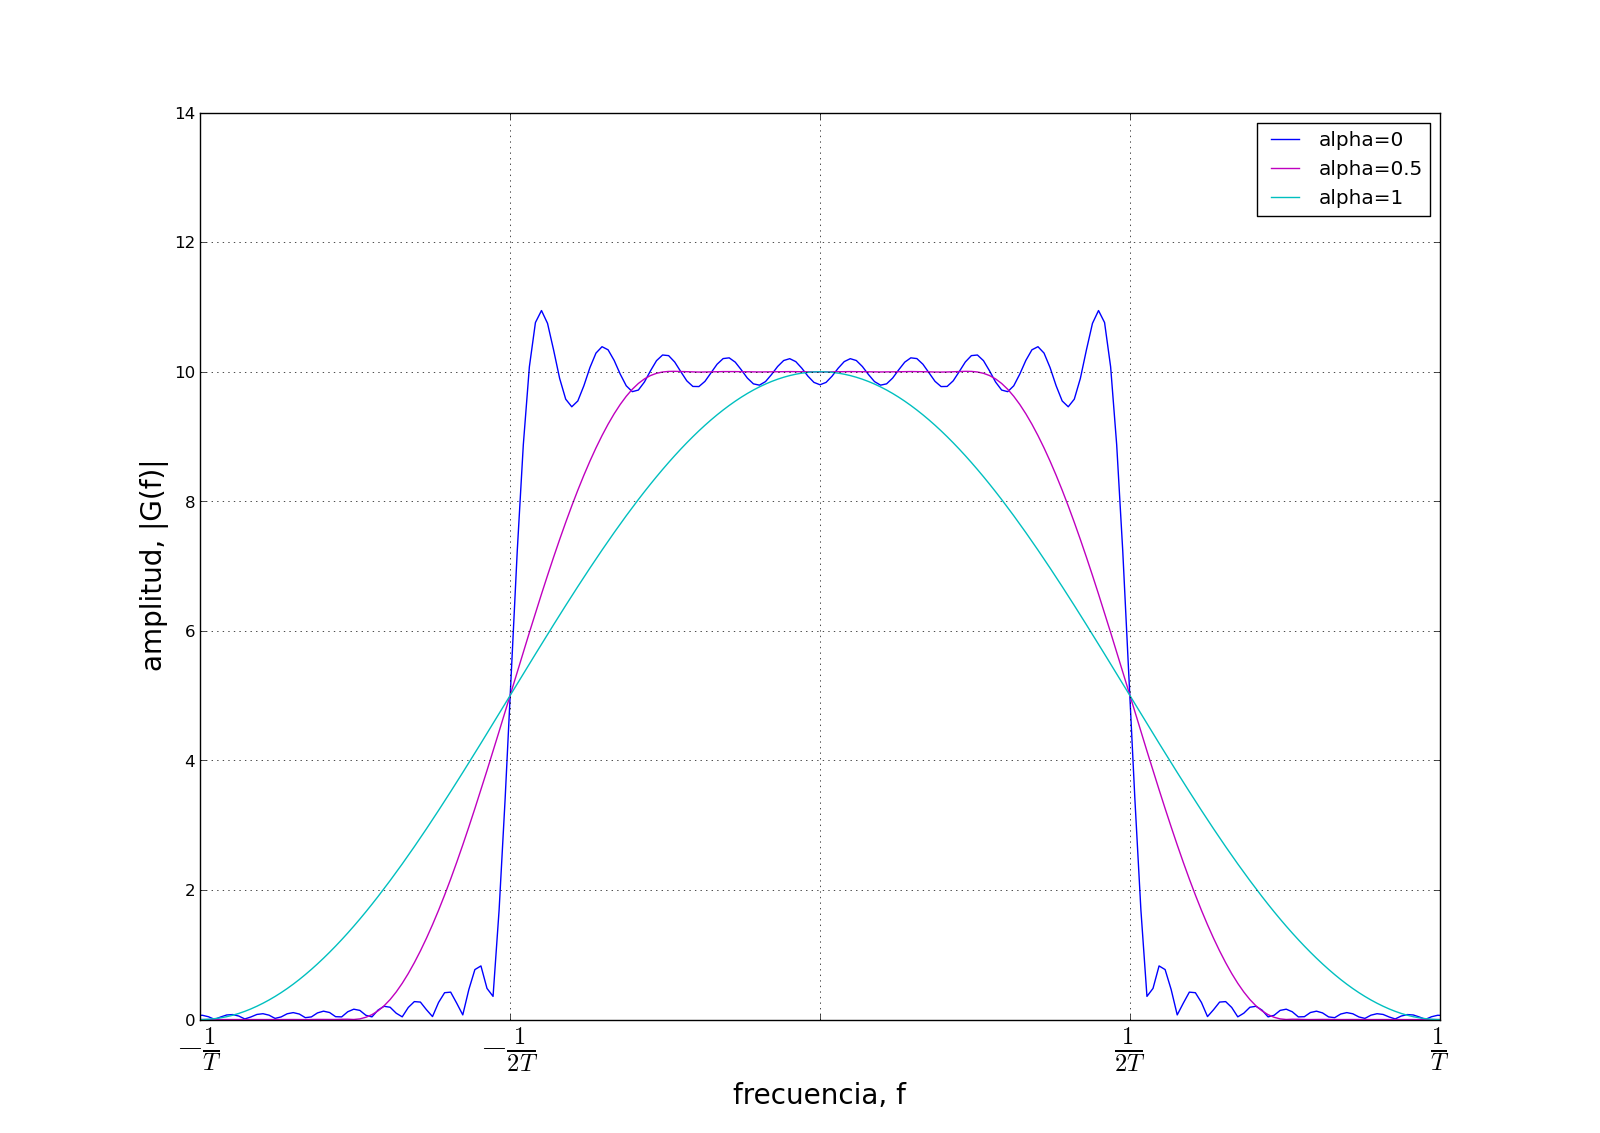
\includegraphics[width=5.9in]{figs/rrcfreq}
  \vspace{0.3in}
  \caption{Representaci\'on en el dominio de la frecuencia de filtros coseno elevado}
  \label{fig:rrcfreq}
\end{figure}

\begin{figure}[htp]
  \centering
  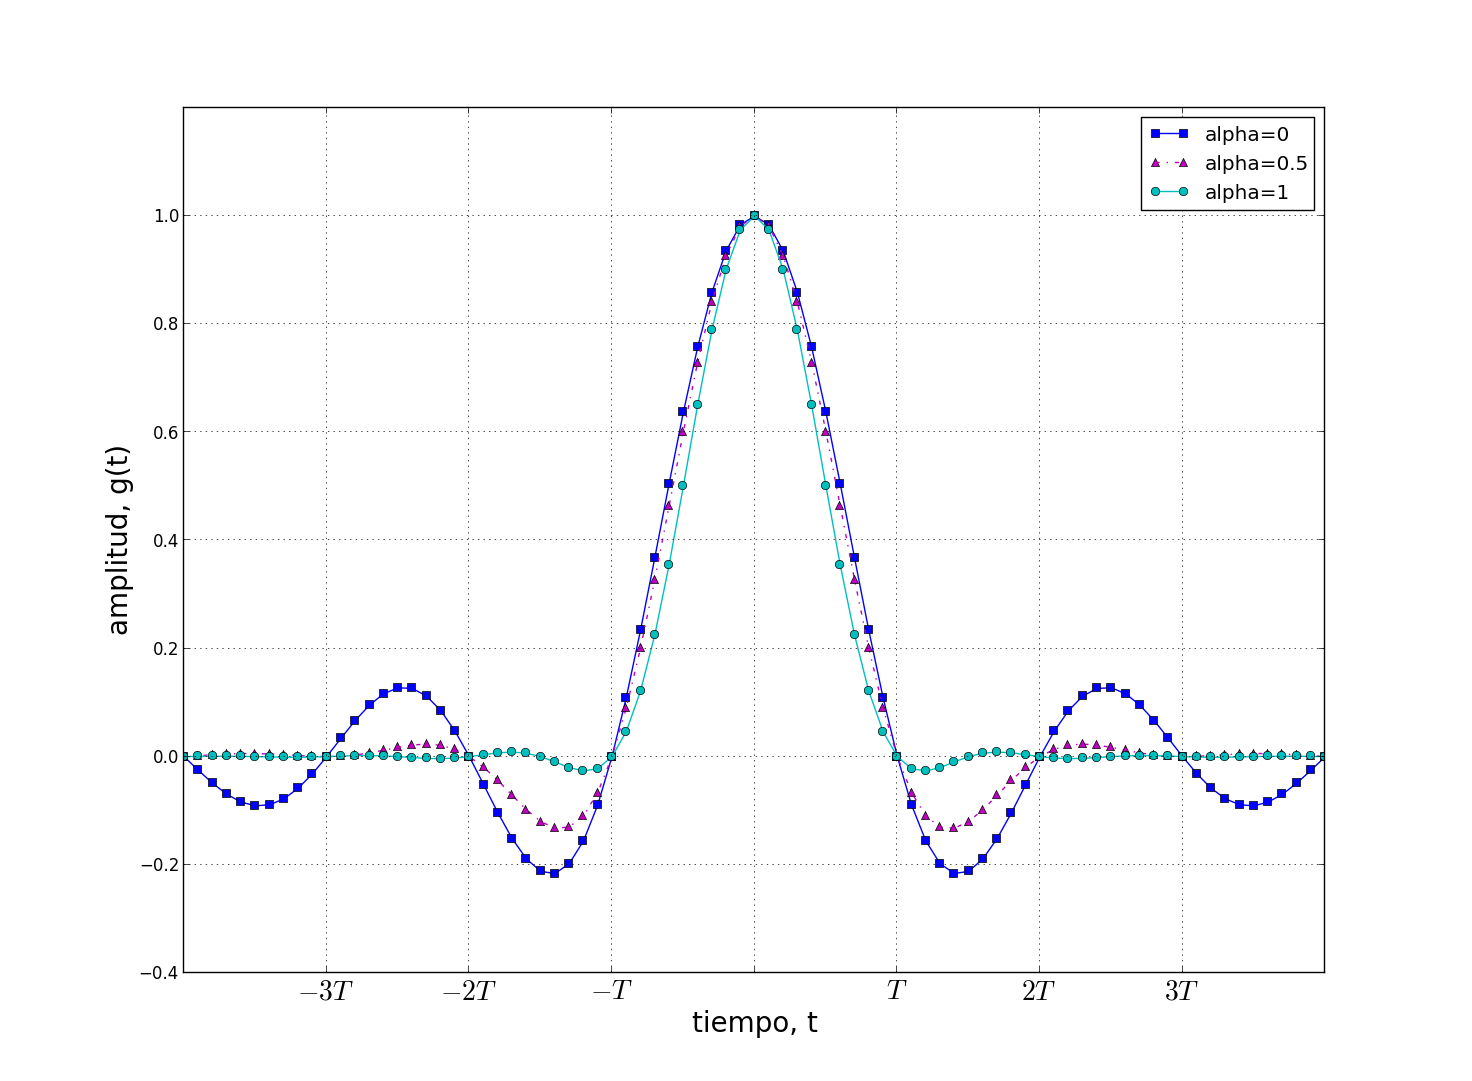
\includegraphics[width=5.9in]{figs/rrctime}
  \vspace{0.3in}
  \caption{Forma de onda en el dominio del tiempo para filtros de coseno elevado}
  \label{fig:rrctime}
\end{figure}

La clase \verb|blks2.dqpsk_mod| representa el modulador DQPSK. Un ejemplo de su uso en un programa sencillo se muestra en el
capitulo \ref{ch:resultados}. La clase se puede configurar de acuerdo a los siguientes par\'ametros de entrada:

\begin{itemize}
  \item \textbf{samples\_per\_symbol}: Especifica la tasa de muestras por s\'imbolo. Acepta valores $\geq 2$.
  \item \textbf{excess\_bw}: Especifica el porcentaje de exceso de ancho de banda que utiliza el filtro RRC.
  \item \textbf{gray\_code}: Bandera booleana que activa o desactiva la codificaci\'on Gray para la generaci\'on de la
  constelaci\'on.
  \item \textbf{verbose}: Especifica si el modulador va imprimir su informaci\'on de configuraci\'on a la consola.
  \item \textbf{log}: Activa la generaci\'on de archivos con los datos que viajan atravez de las aristas del grafo.
\end{itemize} 

% Una vez que los s\'imbolos han sido procesados por el filtro de coseno elevado son enviados al USRP
% por medio del puerto USB. El bloque de salida al USRP se configura de tal manera que el DUC eleve la
% frecuencia de la se\~nal en banda base a una frecuencia intermedia. Esta frecuencia puede ser la que
% se transmite o, dependiendo la tarjeta auxiliar que se est\'e utilizando, puede ser elevada a una
% frecuencia de RF mayor para luego ser transmitida.


\subsection{Modulador DQPSK con filtros polif\'asicos}
Durante el desarrollo de este trabajo los autores de \gnuradio incorporaron al c\'odigo fuente una
versi\'on mejorada del modulador DQPSK que re-implementa algunos bloques del grafo con bancos de
filtros polif\'asicos. Estos filtros son tambien llamados multi tasa (\emph{multirate}) ya que
modifican la frecuencia de muestreo (decimacion e interpolacion) y consisten en un filtro
tradicional (pasa bajas, pasa altas, etc.) y uno o mas componentes que modifican la tasa de muestreo
(decimador o interpolador) \cite{behrouz}. Un ejemplo de estos filtros se muestra en la figura \ref{fig:multirate}.

%NOTA: Para usar la funcion matrix dentro de una subfigura hay que utilizar la opcion ``ampersand replacement'' y cambiar el
% uso del ampersand por algun otro macro. Aqui estamos utilizando \& para mantener consistencia.
\begin{figure}[htp]
  \centering
  \vspace{0.5in}
  \subfloat[Interpolador con factor $L$.]{
  \label{fig:interpol}
  \begin{tikzpicture}[scale=0.8, transform shape]
   \matrix (l) [matrix of nodes, ampersand replacement=\&, column sep=1cm, nodes={draw,
   																				  anchor=center,
   																				  text centered,
   														  						  minimum size=4em},
   				empty/.style={draw=none, fill=white}]
	 { |[empty]| {$x(t)$} \& {$\uparrow L$} \& \filterLP \& |[empty]| {$x'(n)$} \\ };

	 {[start chain, every on chain/.style={join=by ->}]
	 \chainin (l-1-1);
	 \chainin (l-1-2);
	 \chainin (l-1-3);
	 \chainin (l-1-4);
	 };
  \end{tikzpicture}
  }\\
  \subfloat[Decimador con factor $M$.]{
  \label{fig:decimat}
  \begin{tikzpicture}[scale=0.8, transform shape]
  \matrix (d) [matrix of nodes, ampersand replacement=\&, column sep=1cm, nodes={draw,
  													   anchor=center,
  													   text centered,
  													   minimum size=4em},
  			   empty/.style={draw=none, fill=white}]
  	{|[empty]| {$x(t)$} \& \filterLP \& {$\downarrow M$} \& |[empty]| {$x'(n)$} \\ };

  	{[start chain, every on chain/.style={join=by ->}]
  	\chainin (d-1-1);
  	\chainin (d-1-2);
  	\chainin (d-1-3);
  	\chainin (d-1-4);
  	};
  \end{tikzpicture}
  }\\
  \subfloat[Filtro factorial con factor $L/M$.]{
  \label{fig:fractional}
  \begin{tikzpicture}[scale=0.8, transform shape]
  \matrix (d) [matrix of nodes, ampersand replacement=\&, column sep=1cm, nodes={draw,
  													   anchor=center,
  													   text centered,
  													   minimum size=4em},
  			   empty/.style={draw=none, fill=white}]
  	{|[empty]| {$x(t)$} \& {$\uparrow L$} \& \filterLP \& {$\downarrow M$} \& |[empty]| {$x'(n)$} \\ };

  	{[start chain, every on chain/.style={join=by ->}]
  	\chainin (d-1-1);
  	\chainin (d-1-2);
  	\chainin (d-1-3);
  	\chainin (d-1-4);
  	\chainin (d-1-5);
  	};
  \end{tikzpicture}
  }
  \vspace{0.3in}
  \caption{Estructuras basicas de filtros multi tasas.}
  \label{fig:multirate}
\end{figure}

La figura \ref{fig:interpol} muestra la estructura de un interpolador simple con factor de
interpolacion $L$. Este filtro reconstruye una se\~nal $x(n)$ a una taza $L$ veces mas que la taza
de muestreo original. Esto se logra anexando $L-1$ ceros despues de cada muestra y despues se
utiliza un filtro pasa bajas para eliminar las imagenes espectrales que se generan alrededor de la
se\~nal debido a la operacion de \emph{upsampling} \cite{behrouz}.

La figura \ref{fig:decimat} muestra la estructura de un filtro decimador con factor $M$. Aqui el
filtro pasa bajas se utiliza antes del decimador para reducir el ancho de banda de la se\~nal y
prevenir que se genere el efecto alias debido a la reduccion de la frecuencia de muestreo. El
decimador entonces tomara cada $D$ veces muestras e ignorara el resto.

Los filtros anteriores utilizan factores enteros y por lo tanto no se puede realizar interpolaci\'on
o decimaci\'on fraccional \cite{behrouz}. Un tercer filtro combina ambas estructuras para lograr precisamente esto y
se le denomina filtros factoriales $L/M$. Su estructura se muestra en la figura
\ref{fig:fractional}. Aqu\'i el filtro pasa bajas se encuentre entre el bloque de \emph{upsampling} y
el bloque decimador para proporcionar interpolaci\'on a la se\~nal y protecci\'on contra el efecto
alias.

El problema principal con las estructuras anteriores es que no son muy eficientes. El filtro decimador calcula
muchas muestras que eventualmente ser\'an descartadas y el filtro interpolador procesa las muestras de
la se\~nal as\'i como tambi\'en los ceros introducidos por la operaci\'on \emph{upsampling}. Para
solucionar esto se utiliza una estructura de filtros polif\'asicos para lograr que el filtro decimador
e interpolador procesen la se\~nal a la taza de muestreo original y no a la taza modificada. La
estructura del filtro decimador en su descomposici\'on polif\'asica se muestra en la figura
\ref{fig:polydecim}.

\begin{figure}[htp]
  \centering
  \vspace{0.5in}
  \begin{tikzpicture}[scale=0.8, transform shape]
  \matrix (d) [matrix of nodes, column sep=1cm, nodes={draw,
    													   anchor=center,
    													   text centered,
    													   minimum size=3em},
    			   empty/.style={draw=none, fill=white}]
    	{|[empty]| {$x(t)$} & |[coordinate]| & {$\downarrow M$}     & {$H_0(z)$}           & & \\
    	                    & {$z^{-1}$}     &                      &                      & & \\
    	                    & |[coordinate]| & {$\downarrow M$}     & {$H_1(z)$}           & \sumop & |[empty]| {$y(t)$} \\
    	                    &                &                      &                      & & \\
    	                    &                &                      &                      & & \\
    	                    & {$z^{-1}$}     & |[empty]| {$\vdots$} & |[empty]| {$\vdots$} & & \\
    	                    & |[coordinate]| & {$\downarrow M$} & {$H_n(z)$} & & \\
    	                    };
    	\draw (d-1-1) edge (d-1-2);
    	\draw[->] (d-1-2) -- (d-1-3);
    	\draw[->] (d-1-3) -- (d-1-4);
    	\draw[->] (d-1-4) -- (d-3-5);
    	\draw[->] (d-1-2) -- (d-2-2);
    	\draw (d-2-2) edge (d-3-2);
    	\draw[->, dotted] (d-3-2) -- (d-6-2);
    	
    	\draw[->] (d-3-2) -- (d-3-3);
    	\draw[->] (d-3-3) -- (d-3-4);
    	\draw[->] (d-3-4) -- (d-3-5);
    	\draw[->] (d-3-5) -- (d-3-6);
    	
    	\draw (d-6-2) edge (d-7-2);
    	\draw[->] (d-7-2) -- (d-7-3);
    	\draw[->] (d-7-3) -- (d-7-4);
    	\draw[->] (d-7-4) -- (d-3-5);
  \end{tikzpicture}
  \vspace{0.3in}
  \caption{Descomposicion del filtro decimador en su representacion polif\'asica.}
  \label{fig:polydecim}
\end{figure}

La estructura del modulador DQPSK fue modificada con la introducci\'on de estos filtros al c\'odigo fuente. La estructura de
la segunda versi\'on de este bloque jer\'arquico, llamado DQPSK2, se muestra en la figura \ref{fig:dqpsk2}. El bloque
ilustrado de rojo representa la modificaci\'on que se realizo al grafo del bloque jer\'arquico original.

\begin{figure}[htp]
  \centering
  \vspace{0.5in}
  \begin{tikzpicture}[scale=0.8, transform shape]
	\node (data) [grblock] {\footnotesize{Datos codificados}};
	\node (packtounpack) [grblock, right=of data] {\footnotesize{Desempaquetado de bits}}
	edge [<-, very thick] (data);
	\node (map) [grblock, right=of packtounpack] {\footnotesize{Mapeo de constelaci\'on}}
	edge [<-, very thick] (packtounpack);
	\node (difcode) [grblock, right=of map] {\footnotesize{Codificador diferencial}}
	edge [<-, very thick] (map);
	\node (symbols) [grblock, below=of difcode] {\footnotesize{Bloques a s\'imbolos}}
	edge [<-, very thick] (difcode);
	\node (rrc) [grblock, fill=red!30, left=of symbols] {\footnotesize{Re-muestreo arbitrario RRC}}
	edge [<-, very thick] (symbols);
	\node (usrp) [grblock, left=of rrc] {\footnotesize{Salida al USRP}}
	edge [<-, very thick] (rrc);
  \end{tikzpicture}
  \vspace{0.3in}
  \caption{Estructura del modulador DQPSK con filtros polif\'asicos}
  \label{fig:dqpsk2}
\end{figure}

El bloque en rojo de la figura \ref{fig:dqpsk2} implementa un re-muestreador arbitrario utilizando un banco de filtros
polif\'asicos. La tasa de re-muestreo puede ser cualquier n\'umero real $r$ y realiza la operaci\'on construyendo $N$
cantidad de filtros donde $N$ es el factor de interpolaci\'on. El factor $D$ se calcula de la siguiente manera: $D=N/r$.
Utilizando $N$ y $D$ el bloque realiza un muestreo arbitrario con factor $N/D$ que representa un numero racional cercano a
la tasa especificada $r$ y utilizando $N$ cantidad de filtros que se forman el banco de filtros polif\'asicos.

Este modulador se encuentra dentro del mismo paquete \verb|blsk2| que la versi\'on anterior. Los par\'ametros que acepta la
clase son los mismos que se describieron en el apartado \ref{subsec:estrucdqpsk}.

\subsection{Estructura del receptor}
El programa principal del receptor se encuentra en el archivo \verb|benchmark_rx.py|. La estructura del programa es muy
similar a la del transmisor y la diferencia principal es en el uso de una funci\'on auxiliar que maneja el grafo RX y
se encarga de recibir los paquetes que van recibiendo y desplegar su estatus en la consola. Esta funci\'on se puede
modificar para realizar cualquier otra operaci\'on con los paquetes de datos. El c\'odigo de esta funci\'on se muestra
en el listado \ref{ex:callback}. La estructura del receptor se muestra en la figura \ref{fig:grdqpskrx}.

\begin{figure}[htp]
  \centering
  \begin{tikzpicture}[scale=0.8, transform shape]
  	\node (usrp) [grblock] {\footnotesize{USRP}};
  	\node (preselect) [grblock, right=of usrp] {\footnotesize{Filtro pre-selector}}
	edge [<-, very thick] (usrp);
	\node (demod) [grblock, right=of preselect] {\footnotesize{Demodulador DQPSK}}
	edge [<-, very thick] (preselect);
	\node (decod) [grblock, right=of demod] {\footnotesize{Decodificador de paquetes}}
	edge [<-, very thick] (demod);
  \end{tikzpicture}
  \vspace{0.3in}
  \caption{Diagrama a bloques del receptor DQPSK}
  \label{fig:grdqpskrx}
\end{figure}

\begin{lstlisting}[float, label=ex:callback, caption={Funci\'on auxiliar que recibe los paquetes decodificados},
breaklines=true]
    def rx_callback(ok, payload):
        global n_rcvd, n_right
        (pktno,) = struct.unpack('!H', payload[0:2])
        n_rcvd += 1
        if ok:
            n_right += 1

        print "ok = %5s  pktno = %4d  n_rcvd = %4d  n_right = %4d" % (
            ok, pktno, n_rcvd, n_right)
\end{lstlisting}

Al igual que el transmisor, el receptor define un grafo principal con un solo bloque jer\'arquico que encapsula todas las
diversas operaciones del programa (configuraci\'on del USRP, demodulaci\'on y decodificaci\'on de datos) y su
implementaci\'on se mantiene separado en diversos archivos, cada uno con un prop\'osito exclusivo.

La configuraci\'on del USRP se lleva a cabo dentro del archivo \\ \verb|usrp_receive_path.py|. Las operaciones principales
que realiza el grafo de este archivo es configurar la frecuencia central y el factor de decimaci\'on que se va utilizar dentro
del DDC. Igualmente el programa realiza el c\'alculo de la tasa de bits con los par\'ametros que el usuario especifico y si
no se logra la configuraci\'on el programa emite un mensaje de error. Posteriormente, el control se pasa al archivo
\verb|receive_path.py| para la generaci\'on y configuraci\'on del grafo que crea la instancia del demodulador DQPSK.


\subsection{Estructura del demodulador DQPSK}
La estructura del grafo del demodulador DQPSK se muestra en la figura \ref{fig:dqpskdemod}.

\begin{figure}[htp]
	\centering
	\begin{tikzpicture}[scale=0.8, transform shape]
		\node (usrp) [grblock] {\footnotesize{USRP Rx}};
		\node (prescale) [grblock, right=of usrp] {\footnotesize{Pre-escalador \\ $\pm$}}
		edge [<-, very thick] (usrp);
		\node (gain) [grblock, right=of prescale] {\footnotesize{Control autom\'atico de ganancia}}
		edge [<-, very thick] (prescale);
		\node (rrc) [grblock, right=of gain] {\footnotesize{Filtro RRC}}
		edge [<-, very thick] (gain);
		\node (receiver) [grblock, below=of rrc] {\footnotesize{Receptor MPSK \\ (PLL y M\&M)}}
		edge [<-, very thick] (rrc);
		\node (difdecod) [grblock, left=of receiver] {\footnotesize{Decodificador diferencial}}
		edge [<-, very thick] (receiver);
		\node (constel) [grblock, left=of difdecod] {\footnotesize{Decodificador de constelaci\'on}}
		edge [<-, very thick] (difdecod);
		\node (sym) [grblock, left=of constel)] {\footnotesize{Selector de s\'imbolos}}
		edge [<-, very thick] (constel);
		\node (unpack) [grblock, below=of sym] {\footnotesize{Desempaquetado de bits}}
		edge [<-, very thick] (sym);
		\node (data) [grblock, right=of unpack] {\footnotesize{Datos recibidos}}
		edge [<-, very thick] (unpack);
	\end{tikzpicture}
	\vspace{0.3in}
	\caption{Estructura del demodulador DQPSK}
	\label{fig:dqpskdemod}
\end{figure}

La se\~nal que entrega el USRP es multiplicada por una constante para escalarla de su rango completo ,$\pm$16384, a $\pm$1.
Despu\'es se entrega a un controlador autom\'atico de ganancia no causal el cual se encarga de calcular la ganancia requerida en
base al valor absoluto m\'aximo sobre $n$ muestras.

Al igual que el transmisor, el demodulador cuenta con un filtro de coseno elevado con las mismas caracter\'isticas utilizadas en
la etapa de transmisi\'on. El filtro es necesario para completar el acoplamiento ya que individualmente son filtros ra\'iz de
coseno elevado y su respuesta a la frecuencia combinada es la del filtro coseno elevado \cite{sklar} como se muestra en la ecuaci\'on
\ref{eq:rrc}.

\begin{equation}\label{eq:rrc}
H_{rc}(f) = H_{rrc}(f) \cdot H_{rrc}(f)
\end{equation}

El bloque \verb|Receptor MPSK| se encarga de realizar la sincron\'ia de la fase y frecuencia de la se\~nal y del reloj de
s\'imbolos. Esto lo hace en dos etapas las cuales son por medio de un PLL llamado Lazo de Costas y un algoritmo de sincron\'ia de
reloj llamado M\&M (Mueller \& Muller por los nombres de sus autores). El Lazo de Costas encuentra el error en la se\~nal recibida
compar\'andola con su punto de constelaci\'on mas cercano. La frecuencia y la fase de un NCO (Oscilador controlado
num\'ericamente) son actualizados en base a este error. La sincronizaci\'on de s\'imbolos se realiza por medio de una versi\'on
modificada del algoritmo de Mueller y Muller descrita en el art\'iculo t\'ecnico \emph{Optimisation of modified Mueller and Muller
algorithm} publicado el 22 de Junio de 1995. El algoritmo realiza una interpolaci\'on de una muestra (utilizando el NCO del Lazo
de Costas) cada $\mu$ muestras y luego encuentra el error de muestreo basado en el actual y los pasados s\'imbolos y la decisi\'on
tomada sobre las muestras. Para los dos, PLL y M\&M, \gnuradio implementa algoritmos optimizados para BPSK y QPSK pero para 8PSK
utiliza una soluci\'on que los autores le llaman \emph{fuerza bruta} para calcular la distancia m\'inima de los puntos de la
constelaci\'on.

Antes de iniciar con la decodificaci\'on de la constelaci\'on, los bits son decodificados a trav\'es de un decodificador
diferencial utilizando la ecuaci\'on \eqref{eq:difdecod}. El resto de los bloques se encargan de convertir los valores
complejos a bits y decodificar los puntos de la constelaci\'on para luego entregar cada bit individualmente al resto de la aplicaci\'on. 

\subsection{Demodulador DQPSK con filtros polif\'asicos}

Para la segunda versi\'on del c\'odigo que implementa el esquema DQPSK con filtros polif\'asicos las modificaciones se
muestran en la figura \ref{fig:dqpsk2demod}. Los bloques mostrados en rojo representan las modificaciones al grafo original.

\begin{figure}[htp]
	\centering
	\begin{tikzpicture}[scale=0.8, transform shape]
		\node (usrp) [grblock] {\footnotesize{USRP Rx}};
		\node (gain) [grblock, right=of usrp] {\footnotesize{Control autom\'atico de ganancia}}
		edge [<-, very thick] (usrp);
		\node (fll) [grblock, fill=red!30, right=of gain] {\footnotesize{Correcci\'on de frecuencia (FLL)}}
		edge [<-, very thick] (gain);
		\node (rrc) [grblock, fill=red!30, right=of fll] {\footnotesize{Sincronizador de s\'imbolos y RCC}}
		edge [<-, very thick] (fll);
		\node (costas) [grblock, fill=red!30, below=of rrc] {\footnotesize{Lazo de Costas (PLL)}}
		edge [<-, very thick] (rrc);
		\node (difdecod) [grblock, left=of costas] {\footnotesize{Decodificador diferencial}}
		edge [<-, very thick] (costas);
		\node (constel) [grblock, left=of difdecod] {\footnotesize{Decodificador de constelaci\'on}}
		edge [<-, very thick] (difdecod);
		\node (sym) [grblock, left=of constel)] {\footnotesize{Selector de s\'imbolos}}
		edge [<-, very thick] (constel);
		\node (data) [grblock, below=of sym] {\footnotesize{Datos recibidos}}
		edge [<-, very thick] (sym);
	\end{tikzpicture}
	\vspace{0.3in}
	\caption{Estructura del demodulador DQPSK con filtros polif\'asicos.}
	\label{fig:dqpsk2demod}
\end{figure}

Despu\'es de la etapa de control de ganancia el sistema inicia con un FLL (Bucle de Enganche de Frecuencia) el cual se
encarga de generar una se\~nal de referencia con la frecuencia correcta de la portadora. El FLL cubre el ancho de banda superior e
inferior de la se\~nal modulada. Este rango se determina por el factor $\alpha$ (exceso de ancho de banda) de la se\~nal y
las esquinas superior e inferior del ancho de banda son determinadas por la taza de sobre-muestreo (el numero de muestras
por s\'imbolo) y el factor $\alpha$.

El FLL filtra las bandas superior e inferior en $x_u(t)$ y $x_l(t)$ respectivamente \cite{radio}. Estas se combinan para
formar

\begin{equation}\label{eq:ffl1}
cc(t)=x_u(t)+x_l(t)
\end{equation}

y 

\begin{equation}\label{eq:ffl2}
ss(t)=x_u(t)-x_l(t)
\end{equation}

Combinando \eqref{eq:ffl1} y \eqref{eq:ffl2} nos da la se\~nal

\begin{equation}
e(t)=Re\{cc(t) \times ss(t)^*\}
\end{equation}

donde $^*$ es el operador del conjugado complejo. Esta se\~nal error es directamente proporcional a la frecuencia de la
portadora. Despu\'es se crea un lazo de segundo orden utilizando esta se\~nal. El bloque realiza todos estos c\'alculos
internamente dentro de una funci\'on llamada \verb|design_filter()|.

El bloque \emph{Sincronizador de s\'imbolos} realiza sincronizaci\'on de tiempo a se\~nales PAM (Modulaci\'on por Amplitud
de Pulsos) por medio de la minimizaci\'on de la derivada de la se\~nal filtrada, el cual a su vez maximiza el SNR y minimiza el
efecto ISI \cite{radio}. Para lograr esto el bloque construye dos bancos de filtros polif\'asicos; el primero contiene el
filtro de forma de pulso (ejemplo: filtro de coseno elevado). El segundo banco contiene la derivada de los filtros del
primer banco. Si se observa esto desde el dominio del tiempo, el primer banco contiene filtros que tienen una respuesta al impulso
de forma sinc. El objetivo es alinear la se\~nal de salida de tal forma que sea muestreada justamente en el pico de esta
funci\'on. La derivada de la funci\'on sinc es cero en su punto m\'aximo, o sea, $sinc(0)=1$, $sinc(0)'=0$. Este hecho se
utiliza para generar una se\~nal de error $e(n)$. Esta se\~nal entrega un valor proporcional a la distancia con respecto al punto
cero. El bloque utiliza un PLL de segundo orden para lograr que el error llegue a cero.

El tercer bloque rojo simplemente implementa el Lazo de Costas para la correcci\'on de la fase de la se\~nal por separado
(anteriormente lo implementaba dentro de un solo bloque junto con la sincronizaci\'on de s\'imbolos). La clase que la
implementa se llama \verb|gr.costas_loop_cc|. Con esto, esta versi\'on del demodulador realiza la recuperaci\'on de la
portadora en tres etapas: correcci\'on de frecuencia, sincronizaci\'on de s\'imbolos y filtro de forma de pulso por medio de
filtros polif\'asicos y correcci\'on de fase por medio del Lazo de Costas. Una comparaci\'on detallada del rendimiento de
ambos m\'etodos (con y sin filtros polif\'asicos) de demodulaci\'on QPSK se muestra en el siguiente cap\'itulo.
